\documentclass[aspectratio=169]{beamer}

\usetheme{Boadilla}
\usefonttheme{professionalfonts}
\setbeamertemplate{navigation symbols}{}
\setbeamertemplate{itemize items}[circle]
\setbeamertemplate{enumerate items}[default]
\setbeamertemplate{headline}{}

\usepackage[utf8]{inputenc}
\usepackage[T1]{fontenc}
\usepackage{lmodern}
\usepackage{amsmath}
\usepackage{booktabs}
\usepackage{tabularx}
\usepackage{array}
\usepackage{hyperref}
\usepackage[strings]{underscore}
\usepackage{listings}
\usepackage{tikz}
\usetikzlibrary{arrows.meta,positioning,fit,calc,shapes.geometric}
\usepackage{xcolor}

\definecolor{courseblue}{HTML}{12355B}
\definecolor{coursegold}{HTML}{C98A2E}
\definecolor{courseice}{HTML}{EEF3F8}
\definecolor{coursegreen}{HTML}{2F6B4F}
\definecolor{coursegray}{HTML}{4B5563}
\definecolor{codebg}{HTML}{F7F9FC}
\definecolor{codecomment}{HTML}{5E6C84}
\definecolor{codestring}{HTML}{0B6E4F}

\setbeamercolor{palette primary}{bg=courseblue,fg=white}
\setbeamercolor{palette secondary}{bg=coursegold,fg=white}
\setbeamercolor{palette tertiary}{bg=courseblue,fg=white}
\setbeamercolor{palette quaternary}{bg=coursegold,fg=white}
\setbeamercolor{structure}{fg=courseblue}
\setbeamercolor{frametitle}{bg=courseice,fg=courseblue}
\setbeamercolor{title}{fg=courseblue}
\setbeamercolor{block title}{bg=courseblue,fg=white}
\setbeamercolor{block body}{bg=courseice,fg=black}
\setbeamercolor{normal text}{fg=black,bg=white}
\setbeamercolor{alerted text}{fg=coursegold}

\setbeamerfont{footline}{size=\scriptsize}

\setbeamertemplate{footline}{
  \leavevmode
  \hbox{
    \begin{beamercolorbox}[wd=.33\paperwidth,ht=2.8ex,dp=1.2ex,leftskip=0.8em]{palette primary}%
      University of Trieste
    \end{beamercolorbox}%
    \begin{beamercolorbox}[wd=.49\paperwidth,ht=2.8ex,dp=1.2ex,center]{palette tertiary}%
      \coursename{} \textbar{} \coursecode
    \end{beamercolorbox}%
    \begin{beamercolorbox}[wd=.18\paperwidth,ht=2.8ex,dp=1.2ex,right,rightskip=0.8em]{palette secondary}%
      \insertframenumber{} / \inserttotalframenumber
    \end{beamercolorbox}%
  }
}

\hypersetup{
  colorlinks=true,
  linkcolor=courseblue,
  urlcolor=coursegreen
}

\lstdefinestyle{coursepython}{
  language=Python,
  basicstyle=\ttfamily\footnotesize,
  keywordstyle=\color{courseblue}\bfseries,
  commentstyle=\color{codecomment}\itshape,
  stringstyle=\color{codestring},
  showstringspaces=false,
  columns=fullflexible,
  keepspaces=true,
  frame=single,
  framerule=0.6pt,
  rulecolor=\color{courseblue},
  backgroundcolor=\color{codebg},
  xleftmargin=0.4em,
  xrightmargin=0.4em,
  aboveskip=0.4em,
  belowskip=0.2em
}

\newcommand{\coursename}{Data-driven Systems Engineering}
\newcommand{\coursecode}{440MI / 305SM}
\newcommand{\coursefooter}{}

\newcommand{\learninggoals}[1]{
  \begin{block}{Learning goals}
  #1
  \end{block}
}

\newcommand{\repoactivity}[1]{
  \begin{block}{Repo activity}
  #1
  \end{block}
}

\newcommand{\readinglist}[1]{
  \begin{block}{Papers and materials}
  {\footnotesize #1}
  \end{block}
}

\newcommand{\coursecontextframe}[5]{
  \begin{frame}{Course Map and Running Cases}
  \centering
  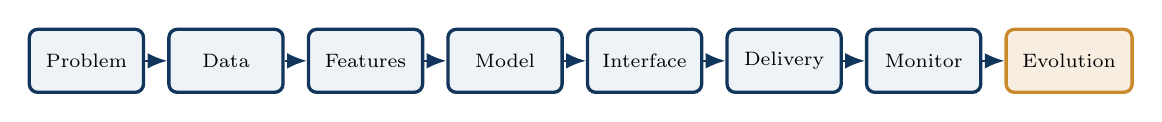
\begin{tikzpicture}[node distance=0.28cm]
  \node[flowbox, minimum width=1.45cm, minimum height=0.8cm] (problem) {\scriptsize Problem};
  \node[flowbox, minimum width=1.45cm, minimum height=0.8cm, right=of problem] (data) {\scriptsize Data};
  \node[flowbox, minimum width=1.45cm, minimum height=0.8cm, right=of data] (features) {\scriptsize Features};
  \node[flowbox, minimum width=1.45cm, minimum height=0.8cm, right=of features] (model) {\scriptsize Model};
  \node[flowbox, minimum width=1.45cm, minimum height=0.8cm, right=of model] (interface) {\scriptsize Interface};
  \node[flowbox, minimum width=1.45cm, minimum height=0.8cm, right=of interface] (delivery) {\scriptsize Delivery};
  \node[flowbox, minimum width=1.45cm, minimum height=0.8cm, right=of delivery] (monitor) {\scriptsize Monitor};
  \node[accentbox, minimum width=1.6cm, minimum height=0.8cm, right=of monitor] (evolution) {\scriptsize Evolution};
  \foreach \a/\b in {problem/data,data/features,features/model,model/interface,interface/delivery,delivery/monitor,monitor/evolution} {
    \draw[arrow] (\a) -- (\b);
  }
  \end{tikzpicture}

  \vspace{0.5em}
  \begin{block}{Today in the course}
  \textbf{Focus:} #1

  \textbf{Bridge:} #2
  \end{block}

  \begin{columns}[T]
  \column{0.48\textwidth}
  \begin{block}{Fraud case}
  {\footnotesize #3}
  \end{block}
  \column{0.48\textwidth}
  \begin{block}{Pasteurization case}
  {\footnotesize #4}
  \end{block}
  \end{columns}

  \vspace{0.3em}
  {\footnotesize \textbf{Course thread:} #5}
  \coursefooter
  \end{frame}
}

\newcommand{\classclosingframe}[4]{
  \begin{frame}{From This Class to the Next}
  \begin{block}{What stays with us}
  #1
  \end{block}

  \begin{columns}[T]
  \column{0.48\textwidth}
  \begin{block}{Project use}
  {\footnotesize #2}
  \end{block}
  \column{0.48\textwidth}
  \begin{block}{Next connection}
  {\footnotesize #3}
  \end{block}
  \end{columns}

  \vspace{0.3em}
  {\footnotesize \textbf{Course thread:} #4}
  \coursefooter
  \end{frame}
}

\tikzset{
  flowbox/.style={
    rounded corners=3pt,
    draw=courseblue,
    fill=courseice,
    very thick,
    minimum width=2.2cm,
    minimum height=0.9cm,
    align=center,
    font=\small
  },
  accentbox/.style={
    rounded corners=3pt,
    draw=coursegold,
    fill=coursegold!15,
    very thick,
    minimum width=2.2cm,
    minimum height=0.9cm,
    align=center,
    font=\small
  },
  arrow/.style={
    -{Latex[length=2.5mm,width=2mm]},
    thick,
    draw=courseblue
  }
}

\usepackage{amssymb}

\title{Class 19: Lab --- Streaming Pasteurization Sensors}
\author{\coursename}
\date{}

\begin{document}

\frame{\titlepage \coursefooter}

\begin{frame}{Agenda}
\begin{itemize}
\item Goal of the lab: from synthetic sensor generation to a live stream that can be consumed.
\item \texttt{synth\_sensors.py}: states, sensors, and the derived feature \texttt{dTdt}.
\item \texttt{serving.py}: the batch, point, and streaming endpoints.
\item Guided exercises: run, inspect, request, stream, and detect drift.
\item What to observe, and common pitfalls.
\end{itemize}
\coursefooter
\end{frame}

\begin{frame}{Lab overview and setup}
\begin{enumerate}
\item From the repository root, install the dependencies: \texttt{pip install -r requirements.txt}.
\item Two files are used: \texttt{pasteurization/synth\_sensors.py} and \texttt{pasteurization/serving.py}.
\item \texttt{synth\_sensors.py} does not depend on Flask; it can be run and inspected on its own.
\item \texttt{serving.py} imports the simulation functions from \texttt{synth\_sensors.py} and exposes them over the Hypertext Transfer Protocol (HTTP).
\end{enumerate}
\coursefooter
\end{frame}

\begin{frame}{Architecture of the lab}
\centering
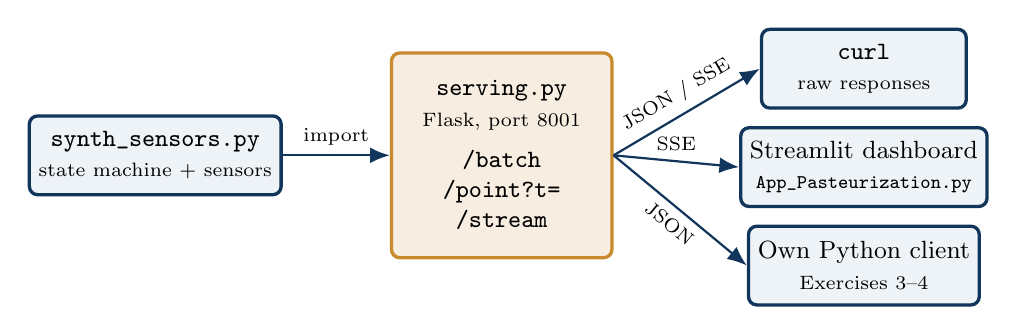
\begin{tikzpicture}[font=\footnotesize, box/.style={flowbox, minimum width=2.6cm, minimum height=1.0cm}]
\node[box] (gen) at (0,0) {\texttt{synth\_sensors.py}\\\scriptsize state machine + sensors};
\node[accentbox, minimum width=2.8cm, minimum height=2.6cm, align=center] (srv) at (4.4,0) {\texttt{serving.py}\\\scriptsize Flask, port 8001\\[0.4em]\texttt{/batch}\\\texttt{/point?t=}\\\texttt{/stream}};
\node[box] (curl) at (9.0,1.1) {\texttt{curl}\\\scriptsize raw responses};
\node[box] (st) at (9.0,-0.15) {Streamlit dashboard\\\scriptsize \texttt{App\_Pasteurization.py}};
\node[box] (own) at (9.0,-1.4) {Own Python client\\\scriptsize Exercises 3--4};
\draw[arrow] (gen) -- node[above, font=\scriptsize] {import} (srv);
\draw[arrow] (srv.east) -- node[above, sloped, font=\scriptsize] {JSON / SSE} (curl.west);
\draw[arrow] (srv.east) -- node[above, font=\scriptsize] {SSE} (st.west);
\draw[arrow] (srv.east) -- node[below, sloped, font=\scriptsize] {JSON} (own.west);
\end{tikzpicture}
\vspace{0.6em}
\begin{itemize}\footnotesize
\item \texttt{/batch} returns one complete simulated batch as a JSON array; \texttt{/point?t=} returns a single reading; \texttt{/stream} replays one batch as Server-Sent Events (SSE), one event per second.
\item The generator has no knowledge of HTTP, and the clients have no knowledge of the simulation: each layer can be tested in isolation.
\end{itemize}
\coursefooter
\end{frame}

\begin{frame}[fragile]{Sensors and states in the code}
\begin{lstlisting}[style=coursepython]
# Sensors (7): Temperature, pH, Kappa, Mu, Tau, Q_in, Q_out, P
# Derived: dT/dt

PROD_RANGES = {
    "Idle":      (60, 120),
    "Fill":      (30, 60),
    "HeatUp":    (30, 45),
    "Hold":      (15, 25),
    "Cool":      (30, 60),
    "Discharge": (60, 120),
}
\end{lstlisting}
\begin{itemize}
\item From \texttt{pasteurization/synth\_sensors.py}: the docstring counts seven sensors, but inflow and outflow are separate channels, so each sample is $\mathbf{x}_t \in \mathbb{R}^{8}$, plus the derived \texttt{dTdt}.
\item Six production states, each with a duration drawn uniformly from the given range (in seconds) for every batch.
\end{itemize}
\coursefooter
\end{frame}

\begin{frame}{The batch lifecycle as a state machine}
\centering
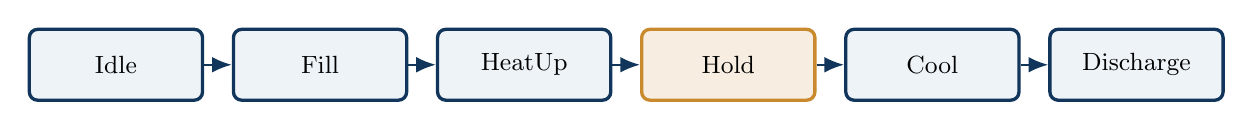
\begin{tikzpicture}[node distance=0.35cm, every node/.append style={minimum width=1.75cm}]
\node[flowbox] (idle) {\small Idle};
\node[flowbox, right=of idle] (fill) {\small Fill};
\node[flowbox, right=of fill] (heat) {\small HeatUp};
\node[accentbox, right=of heat] (hold) {\small Hold};
\node[flowbox, right=of hold] (cool) {\small Cool};
\node[flowbox, right=of cool] (disch) {\small Discharge};
\foreach \a/\b in {idle/fill,fill/heat,heat/hold,hold/cool,cool/disch} {
  \draw[arrow] (\a) -- (\b);
}
\end{tikzpicture}
\vspace{0.6em}
\begin{itemize}
\item Each function \texttt{seg\_*} in \texttt{synth\_sensors.py} generates the signals of exactly one state.
\item The sequence of states is fixed; only the durations are random. The state is therefore a deterministic function of the time elapsed since the start of the batch, given the sampled durations.
\end{itemize}
\coursefooter
\end{frame}

\begin{frame}{Exercise 1: generate and inspect a batch}
\begin{enumerate}
\item Run \texttt{python synth\_sensors.py} from the directory \texttt{pasteurization/}; it simulates 1{,}000 batches (about 324{,}000 samples, a few seconds).
\item Open \texttt{synthetic\_pasteurization\_signals.csv} and verify that the column \texttt{state} contains exactly the six states, in the expected order within each \texttt{batch\_id}.
\item Plot \texttt{T} and \texttt{dTdt} for a single \texttt{batch\_id} and identify the phases HeatUp and Cool.
\item Verify that \texttt{dTdt} changes sign where the temperature trend reverses.
\end{enumerate}
\coursefooter
\end{frame}

\begin{frame}{Exercise 1: expected result}
\centering
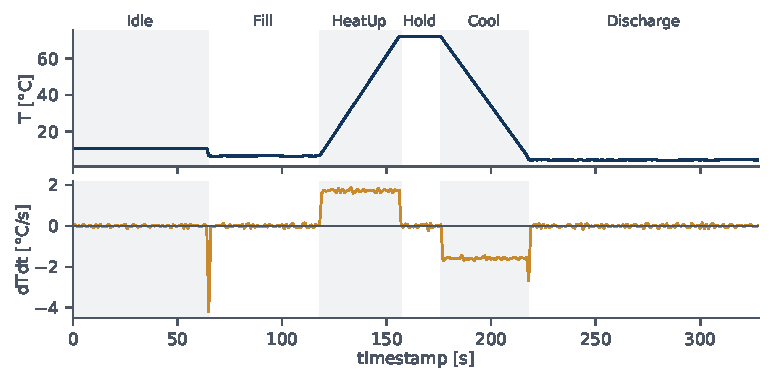
\includegraphics[width=0.82\textwidth,height=0.58\textheight,keepaspectratio]{images/class19_expected_batch.pdf}

\vspace{0.2em}
\begin{itemize}\footnotesize
\item One batch: the temperature rises during HeatUp, stays at the set point of 72\,°C during Hold, and falls during Cool.
\item \texttt{dTdt} is approximately constant and positive during HeatUp, negative during Cool, and close to zero elsewhere; isolated spikes occur where a state begins with a jump in temperature (e.g.\ at the start of Fill).
\end{itemize}
\coursefooter
\end{frame}

\begin{frame}[fragile]{The derived feature in the code}
\begin{lstlisting}[style=coursepython]
def simulate_batch(bid, start_time=0.0):
    ...
    frames = simulate_production_cycle(pdur, ctx)
    df, t = to_df(frames, start_time, bid)
    df["dTdt"] = df["T"].diff().fillna(0.0) / DT
    return df, t
\end{lstlisting}
\begin{itemize}
\item \texttt{dTdt} is the backward finite difference $(T_t - T_{t-1})/\Delta t$, the rate-of-change feature constructed in Class 15.
\item It is causal: it uses only the current and the previous sample, so it can also be computed online on the stream.
\end{itemize}
\coursefooter
\end{frame}

\begin{frame}{Exercise 2: serve the simulation over HTTP}
\begin{enumerate}
\item Start the Flask service: \texttt{python serving.py} (port 8001).
\item Request a complete simulated batch: \texttt{GET /batch}.
\item Request a single reading: \texttt{GET /point?t=45}, then an invalid one: \texttt{GET /point?t=abc}.
\item Request \texttt{GET /point?t=120} several times and compare the returned \texttt{state}.
\end{enumerate}
\vspace{0.4em}
\begin{block}{What to explain}
At $t = 120$\,s the service returns sometimes Fill and sometimes HeatUp: every request samples new phase durations. The endpoint is stateless, so successive points do not belong to the same batch.
\end{block}
\coursefooter
\end{frame}

\begin{frame}[fragile]{Exercise 2: expected responses}
\begin{columns}[T]
\column{0.5\textwidth}
\textbf{\footnotesize\texttt{GET /point?t=45}} {\scriptsize (status 200)}
\begin{lstlisting}[basicstyle=\ttfamily\scriptsize, columns=fullflexible, keepspaces=true, frame=single, backgroundcolor=\color{codebg}, rulecolor=\color{courseblue!40}]
{
  "Kappa": 4.653,  "Mu": 2.229,
  "P": 1.135,      "Q_in": 0.0,
  "Q_out": 0.0,    "T": 10.033,
  "Tau": 0.213,    "dTdt": -0.004,
  "pH": 6.649,
  "state": "Idle", "timestamp": 45.0
}
\end{lstlisting}
\column{0.46\textwidth}
\textbf{\footnotesize\texttt{GET /point?t=abc}} {\scriptsize (status 400)}
\begin{lstlisting}[basicstyle=\ttfamily\scriptsize, columns=fullflexible, keepspaces=true, frame=single, backgroundcolor=\color{codebg}, rulecolor=\color{courseblue!40}]
{
  "error": "Invalid t parameter"
}
\end{lstlisting}
\vspace{0.3em}
\begin{itemize}\footnotesize
\item \texttt{GET /batch} returns a JSON array of about 300--360 such objects, one per second of the batch, with an additional field \texttt{batch\_id}.
\end{itemize}
\end{columns}
\vspace{0.4em}
{\scriptsize Responses captured from \texttt{serving.py}; values rounded to three decimals and keys arranged in two columns for readability. Numerical values differ at every request.\par}
\coursefooter
\end{frame}

\begin{frame}[fragile]{Serving a single point in the code}
\begin{lstlisting}[style=coursepython]
@app.route("/point")
def point():
    try:
        t = float(request.args.get("t", 0))
    except ValueError:
        return jsonify({"error": "Invalid t parameter"}), 400

    data = simulate_point(t)
    return jsonify(data)
\end{lstlisting}
\begin{itemize}
\item From \texttt{pasteurization/serving.py}: the input is validated, and an invalid value returns the status code 400 (Bad Request) with an error message instead of an exception.
\item \texttt{simulate\_point} draws a new timeline at every call, which explains the behaviour observed in Exercise 2.
\end{itemize}
\coursefooter
\end{frame}

\begin{frame}{Exercise 3: consume the live stream}
\begin{enumerate}
\item With \texttt{serving.py} running, request \texttt{curl -N http://localhost:8001/stream}.
\item Observe one JSON event per second in the Server-Sent Events (SSE) format: each event is a line \texttt{data: \{\dots\}} followed by a blank line.
\item Alternatively, run \texttt{streamlit run streamlit/Main.py} and open the Pasteurization page, which consumes the same endpoint.
\item Compare the raw output of \texttt{curl} with the plots of the dashboard.
\end{enumerate}
\coursefooter
\end{frame}

\begin{frame}[fragile]{The streaming endpoint in the code}
\begin{lstlisting}[style=coursepython]
@app.route("/stream")
def stream():
    df, _ = simulate_batch(BATCH_ID)

    def generate():
        for _, row in df.iterrows():
            yield f"data: {json.dumps(row.to_dict())}\n\n"
            time.sleep(STREAM_DT)

    return Response(generate(), mimetype="text/event-stream")
\end{lstlisting}
\begin{itemize}
\item From \texttt{pasteurization/serving.py}: a complete batch is simulated first and then replayed at one row per second as an event stream.
\item Unlike \texttt{/point}, the stream is internally consistent: all events belong to one simulated batch.
\end{itemize}
\coursefooter
\end{frame}

\begin{frame}[fragile]{Writing your own stream client}
\begin{lstlisting}[style=coursepython]
import json, requests

URL = "http://localhost:8001/stream"
with requests.get(URL, stream=True, timeout=10) as r:
    for line in r.iter_lines():
        if line.startswith(b"data: "):
            event = json.loads(line[len(b"data: "):])
            print(event["timestamp"], event["state"], round(event["T"], 2))
\end{lstlisting}
\begin{itemize}
\item \texttt{stream=True} keeps the connection open; \texttt{iter\_lines} yields each line as soon as it arrives.
\item Each SSE event is a line starting with \texttt{data: }, followed by a blank separator line; the payload after the prefix is JSON.
\item Expected output: one line per second, e.g.\ \texttt{0.0 Idle 8.74}, \texttt{1.0 Idle 8.7}, \dots
\end{itemize}
\coursefooter
\end{frame}

\begin{frame}{What to observe while streaming}
\begin{itemize}
\item The states follow the fixed order Idle, Fill, HeatUp, Hold, Cool, Discharge.
\item \texttt{dTdt} is close to zero during Idle and Hold, positive during HeatUp, and negative during Cool.
\item \texttt{Q\_in} is non-zero only during Fill; \texttt{Q\_out} only during Discharge.
\item Every sensor remains within the fixed axis ranges of the Streamlit dashboard.
\end{itemize}
\coursefooter
\end{frame}

\begin{frame}{Common pitfalls in this lab}
\begin{itemize}
\item \textbf{Connection settings:} the IP address and port in the dashboard sidebar (default \texttt{127.0.0.1:8001}) must match the machine where \texttt{serving.py} runs.
\item \textbf{Port conflicts:} check that no other process is already bound to port 8001.
\item \textbf{Concurrency:} \texttt{serving.py} runs Flask with \texttt{threaded=True}; without it, an open \texttt{/stream} connection would block every other request.
\item \textbf{Non-reproducible responses:} \texttt{/stream} simulates a new batch at every call, and \texttt{/point} a new timeline at every request; two clients never receive identical data.
\end{itemize}
\coursefooter
\end{frame}

\begin{frame}[fragile]{Exercise 4: detect an injected drift (Class 18)}
\begin{lstlisting}[style=coursepython, basicstyle=\ttfamily\scriptsize]
import requests, pandas as pd
from river import linear_model, optim, preprocessing, drift

URL = "http://localhost:8001/batch"
frames = [pd.DataFrame(requests.get(URL).json()) for _ in range(30)]
stream = pd.concat(frames, ignore_index=True)
start = sum(len(f) for f in frames[:15])     # drift begins with batch 16

model = preprocessing.StandardScaler() | linear_model.LinearRegression(
    optimizer=optim.SGD(0.01))
adwin = drift.ADWIN(delta=0.002)
for i, e in stream.iterrows():
    mu = e["Mu"] + (0.4 if i >= start else 0.0)   # injected product change
    y_pred = model.predict_one({"T": e["T"]}) or 0.0
    model.learn_one({"T": e["T"]}, mu)
    adwin.update(abs(mu - y_pred))
    if adwin.drift_detected:
        print(f"drift detected at sample {i} (injected at {start})")
\end{lstlisting}
\begin{itemize}\footnotesize
\item Thirty batches are requested from \texttt{/batch} (no waiting) and processed row by row as a stream; the viscosity is shifted by 0.4\,cP from batch 16 on.
\end{itemize}
\coursefooter
\end{frame}

\begin{frame}{Exercise 4: questions}
\begingroup\small
Report the detection delay and every alarm raised before the injection. In ten test runs, the drift was detected 28--54 samples after the injection; one or two alarms during the initial learning phase (roughly the first 1{,}500 samples) are expected.
\par\endgroup
\vspace{0.3em}
\begin{enumerate}\small
\item Why is \texttt{/batch} used instead of \texttt{/stream}? Estimate how long the same experiment would take through \texttt{/stream}.
\item Why do alarms appear during the initial learning phase, and why should they be ignored?
\item Reduce the shift to 0.1\,cP and then to 0.05\,cP: how do the detection delay and the detection rate change?
\item Repeat the experiment with only four batches and the injection after batch 2. Explain why the drift is rarely detected (hint: compare with the learning curve of the online model).
\item Replace the sudden shift by a gradual one (e.g.\ $+0.4\,$cP reached linearly over five batches) and compare the delay.
\end{enumerate}
\coursefooter
\end{frame}

\begin{frame}{Repository connections}
\repoactivity{
\begin{itemize}
\item \texttt{pasteurization/synth\_sensors.py} and \texttt{pasteurization/serving.py}: the generator and the service used throughout the lab.
\item \texttt{streamlit/pages/App\_Pasteurization.py}: the client that consumes \texttt{/stream} and plots every sensor live.
\end{itemize}
}
\coursefooter
\end{frame}

\begin{frame}{Papers and materials}
\readinglist{
\fontsize{6.8}{8.2}\selectfont
\begin{columns}[T]
\column{0.5\textwidth}
\begin{itemize}\setlength{\itemsep}{1pt}
\item Fielding, R.\,T. (2000). \emph{Architectural Styles and the Design of Network-based Software Architectures}. PhD thesis, University of California, Irvine.
\item WHATWG. \href{https://html.spec.whatwg.org/multipage/server-sent-events.html}{HTML Living Standard: Server-sent events}.
\end{itemize}
\column{0.5\textwidth}
\begin{itemize}\setlength{\itemsep}{1pt}
\item Documentation: \href{https://flask.palletsprojects.com/en/stable/}{Flask} (including the \href{https://flask.palletsprojects.com/en/stable/tutorial/}{tutorial}); \href{https://docs.streamlit.io/}{Streamlit}; \href{https://pandas.pydata.org/docs/}{pandas}.
\end{itemize}
\end{columns}
}
\coursefooter
\end{frame}

\begin{frame}{Take-away message}
\vfill
\centering
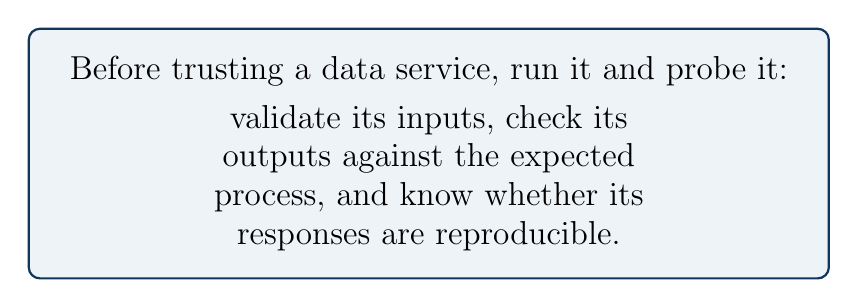
\begin{tikzpicture}
\node[fill=courseice, draw=courseblue, thick, rounded corners=4pt, inner sep=10pt, text width=0.78\textwidth, align=center, font=\large] {Before trusting a data service, run it and probe it:\\[0.3em] validate its inputs, check its outputs against the expected\\ process, and know whether its responses are reproducible.};
\end{tikzpicture}

\vfill
{\Large\bfseries\color{courseblue} Thank you for your attention.}

\vspace{0.4em}
{\small\color{coursegray} Next: Class 20 --- model deployment and prediction serving.}
\vfill
\coursefooter
\end{frame}

\end{document}
